\section{Indoor Technologies}
\label{sec:indoortech}

When looking at the state of indoor positioning systems, it's clear that there isn't one technology that is better than all of the others. As so it's important to look at each of the possible technologies individually and assess its benefits and drawbacks as well as their performance.

In this chapter many existant indoor positioning technologies are analysed. The most pertinent ones, RFID, Wi-Fi, Infrared and UWB, are explained in a more detailed manner in subsections \ref{subsec:rfid}, \ref{subsec:wifi}, \ref{subsec:ir} and \ref{subsec;uwb} respectively, while less utilized technologies are described in subsection \ref{subsec:others}. For each of the present technologies a description is provided about their nature, tags and pros and cons, all of which is complemented with at least one existant system that makes use of the specific technology being described. 


\subsection{RFID}
\label{subsec:rfid}

\ac{RFID} is a technology for storing and retrieving data through electromagnetic transmission to an RF compatible integrated circuit. A \ac{RFID} system is composed by three components: readers, tags and the communication between both. The reader is capable of reading the data that is being emitted from \ac{RFID} tags via radio waves and the data usually consists of the tag's unique identification number which can be related to the tag's available position information in order to obtain the user's position. This communication is achieved by having a well-defined radio frequency and protocol which allows for reading and transmitting data. The \ac{RFID} tags can be of two types: active or passive.

Active tags are small transcievers equiped with an internal battery, which makes them heavier and more costly while allowing for longer detection ranges when compared to their counter-parts. These tags are suited for identification of important units moving through rough processes or positioning in system where location estimation is often carried out through fingerprinting on \ac{RSSI}.
Passive tags are operated without the need of a battery since they are capable of receiving enough energy in the form of radio frequency waves from nearby \ac{RFID} scanners in order to transmit back the answers. These tags are used to replace the barcode technology since they are much lighter, smaller and less expensive than the active tags which allows for a relative inexpensive installation and low maintenance caused by not having batteries. One of its drawbacks is that their range is very limited, circa 2 meters, which demands for higher density of tag deployment.

\ac{RFID}'s biggest advantages are the non required \ac{LOS} characteristics, their capability of working at high speeds and their relative low cost. As such this technology is often used for tracking objects in automobile assembly industry or warehouse management and tracking of people or animals.
One of its most relevant projects is the SpotON \cite{spoton}, a tagging technology for three dimensional location sensing based on radio signal strength analysis. The tags used are custom devices that operate either standalone or as a plug in card enabling larger devices tot ake advantage of location-sensing technology. They are low power, small and capable of being accurate while having the computing capacity for relevant tasks such as caching, authentication, among others. SpotON tags utilize the received \ac{RSSI} as a metric for obtaining inter-tag distance.
Another important project using \ac{RFID} is LANDMARC\cite{landmarc} which utilizes active tags to produce a location sensing system for locating objects inside buildings. Its objective was to demonstrate that active tags can infact be viable and cost-efficient for indoor location sensing. One of the problems found was that the hardware wasn't capable of providing \ac{RSSI} readings, as such the used readers scan through eight discrete power levels in order to estimate the \ac{RSSI}. This scanning coma at the cost of a significant time period. By placing the readers in known positions, the area that is being analyzed can be divided into sub-regions with each being identified by the subset of readers that cover it, which can be visualized in figure \ref{fig:land}. Given an RFID tag, based on the subset of readers that can detect it, the system is capable of associating the tag with a known sub-region. LANDMARC increased the accuracy without placing more
readers by employing extra fixed location reference tags for location calibration.

\begin{figure}[H]
	\centering
		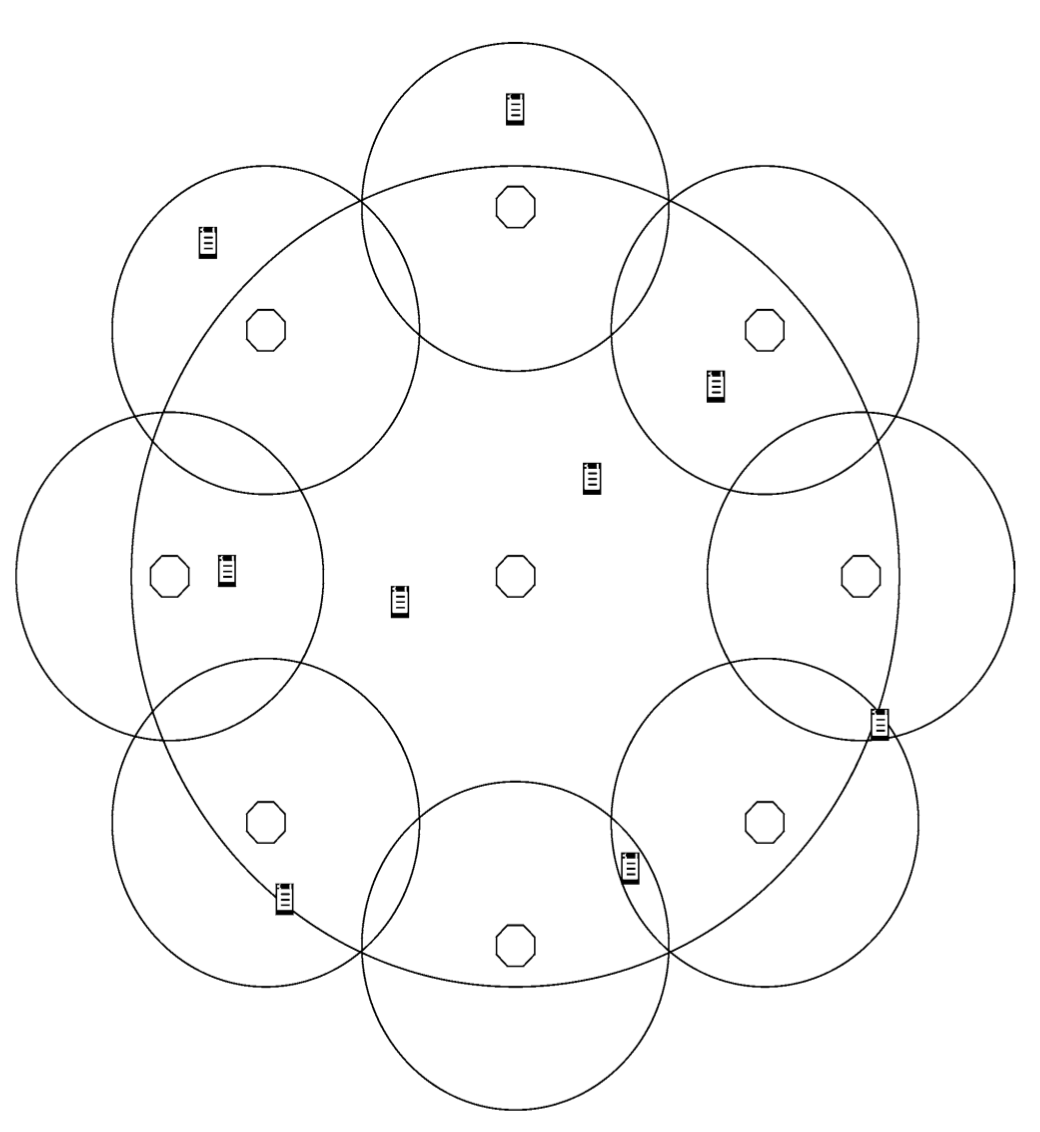
\includegraphics[width=0.5\linewidth]{2.Chapter/landmarc-regions.png}
	\caption[Landmarc deployment showing sub-regions (Ref \cite{landmarc}) ]{Landmarc deployment showing sub-regions (Ref \cite{landmarc})}
	\label{fig:land}
\end{figure}


\subsection{WLAN / Wi-Fi}
\label{subsec:wifi}

\ac{WLAN}is a technology that can be used to estimate the location of a mobile user that resides inside the network. Nowadays Wi-Fi positioning systems have become the most widespread approach for indoor location systems since \ac{WLAN} acess points are readily available in many indoor environments and any Wi-Fi compatible device (smartphones, laptops,tablets) can be located without the need of installing extra software or manipulating the hardware. Its popularity is also due to its range of 100 to 50 meters, which is better than \ad{RFID} and BLE's range, and since \ac{LOS} isn't required. One issue of \ac{WLAN} signals is that they suffer attenuation from static environment such as walls and movement of furniture and doors. In these kind of systems position computation is obtained through TOA, AOA, RSS, and CSI, which are properly analyzed in section \ref{sec:techniques}, with multiple existing projects for each one of the existant methods. The most widely used is the \ac{RSSI}, which suffers from severe multipath effects leading to propagation model failures and as such inaccuracy in distance measurement. With these problems in mind a technique called RSSI-based fingerprinting is often used in order to improve performance.
Most recently an alternative to RSSI has been researched called \ac{CSI}. \ac{CSI} is widely available on commercial products and it represents the channel conditions over individual OFDM subcarriers across the \ac{PHY} layer. One of the improvements is that instead of obtaining one \ac{RSSI} value per packet, multiple \ac{CSI} values can be obtained from multiple subcarriers at a time. FILA \cite{fila} was a project that attempted to use \ac{CSI} for locating targets in complicated indoor environments where RSSI wasn't reliable due to multipath. This system is capable of extracting the \ac{LOS} path for distance calculating through time-domain multipath mitigation and frequency-domain fading compensation and with a simple trilateration calculation they were able to achieve a much better performance than with \ac{RSSI} for these kind of scenarios. The performance comparison showing the differences in temporal stability between \ac{RSSI} and \ac{CSI} can be seen on figure \ref{fig:fila}.

\begin{figure}[H]
	\centering
		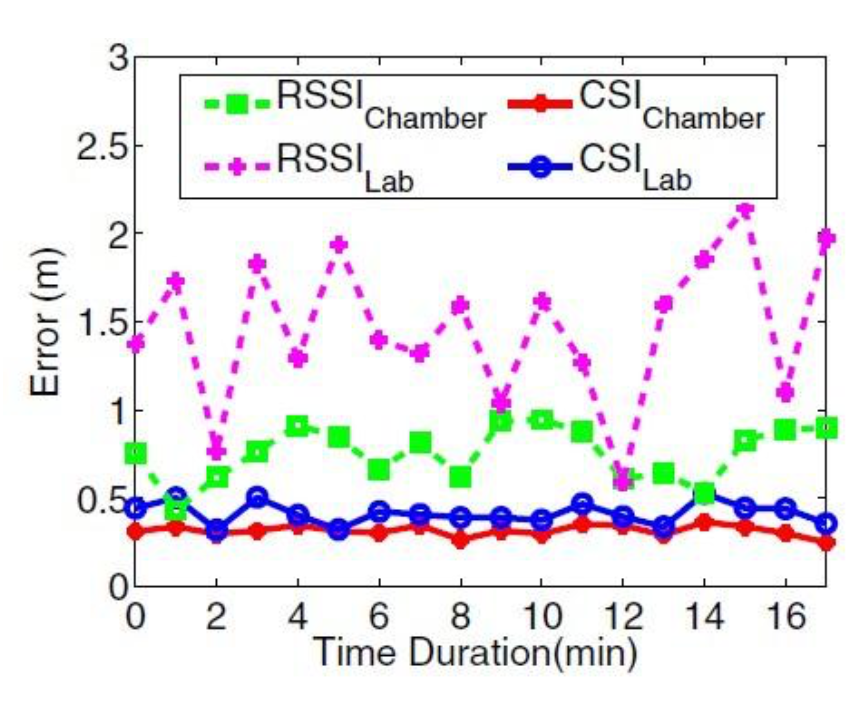
\includegraphics[width=0.5\linewidth]{2.Chapter/fila-comparison.png}
	\caption[Comparison of temporal stability (Ref \cite{fila}) ]{Comparison of temporal stability (Ref \cite{fila})}
	\label{fig:fila}
\end{figure}

\subsection{Infrared}
\label{subsec:ir}

\ac{IR} systems are one of the most common position system that utilize wireless technology that has been used to track objects or people. \ac{IR} wavelengths are invisible to the human eye under most circumstances, making this technology less intrusive than those which are visible. This technology is widely available in various commom devices such as mobile phones, PDA's and Tv's and requires \ac{LOS} communication between receiver and transmitter, preferably without interference from strong light sources. These types of system utilize small, lightweight and easily wearable devices which have the downside of having privacy/security issues. One of the most relevant systems based on \ac{IR} is the Active Badge system which is described in section \ref{sec:related}. There are three methods of exploiting infrared signals: Through active beacons, infrared imaging or artificial light sources.

The active beacon's approach is the one utilized by the active badge system and it involves placing fixed \ac{IR} beacons on known positions. The density of deployment of beacons depends on the objective of the system but if the required is a room-based location, i.e. being able to tell in which room a user is located, a beacon per room should be enough.

Infrared imaging, also known as passive \ac{IR} systems, makes use of sensors operating in the \ac{IR} spectrum which are capable of obtaining a complete image of the surrounding from thermal emissions. This approach doens't require the deployment of any extra hardware or tag for determining the temperature of objects or people but it does get compromised in the presence of strong radiation from the sun. Some known equipments that utilize this approach are thermal cameras, infrared sensors for motion detection or thermocouples used to measure temperature contact free. 

\ac{IR} systems based on artificial light sources are a good alternative to the ones that operate on the visible spectrum. A very well known example is the microsoft Kinect system which uses continuously‐projected infrared structured light to capture 3D scene information	with an	infrared camera. This system is capable of tracking a person's movement up to 3.5 meters with a precision of a few centimeters. 


\subsection{Ultra-Wideband}
\label{subsec:uwb}

\ac{UWB} is a radio technology aimed at short-range high-bandwidth communication. Its best characteristics are its capacity of being resistant to multipath and to some degree being capable of penetrating building materials, such as concrete and wood, with low power consuption. Both these factors allow \ac{UWB} to achieve high positioning accuracy while the latter enables to adress the range in non line-of-sight conditions and makes inter-room ranging possible. Being able to penetrate building material creates precision issues due to the increase in data complexity, making data interpretation one of the biggest challenges to be faced. The usual structure of a \ac{UWB} system has a stimulus radio wave generator and receivers which capture the propagated and scattered waves and it has four types of methods for position calculation.
The first one, passive \ac{UWB}, attemps to track objects or people through signal reflection. This method doesn't require any sort of tag to be carried by the user or attached to the object and requires only at least on emitter and a few listenners to obtain a location. Since the locations of the antennas as known and it is possible to estimate the distance from user to listener through \ac{ToA} or \ac{TDoA} multilateration, the user's location can be computed.
The remaining methods are Direct Ranging and Fingerprinting. The first one simply requires the users to wear active tags and uses differente measures based on time to compute distances which are then worked by lateration techniques in order to produce the user's location. The second one works like a regular fingerprinting method except that it utilizes Channel Impulse Response (CIR) instead of \ac{RSSI}. This kind of fingerprinting has the possibility of being more accurate while being usable in non \ac{LOS} scenarios. On the downside it requires time synchronization.
One commercial example of this technology is Ubisense \cite{ubisense}, a system capable of tracking active tags equiped with batteries which have a conventional RF transciever and a \ac{UWB} trasmitter. The system requires a setup deployment of a network of Ubisensors, with fixed positions throughout the area to be covered and networked using Ethernet. Each sensor has a RF transciever and  phased array of \ac{UWB} receivers. These sensors use a combination of \ac{TDoA} and \ac{AoA} techniques to determine the tags location, achieving an accuracy of 15 cm in a typical open environment. The system's setup can be visualized on figure \ref{fig:ubisense}.


\begin{figure}[H]
	\centering
		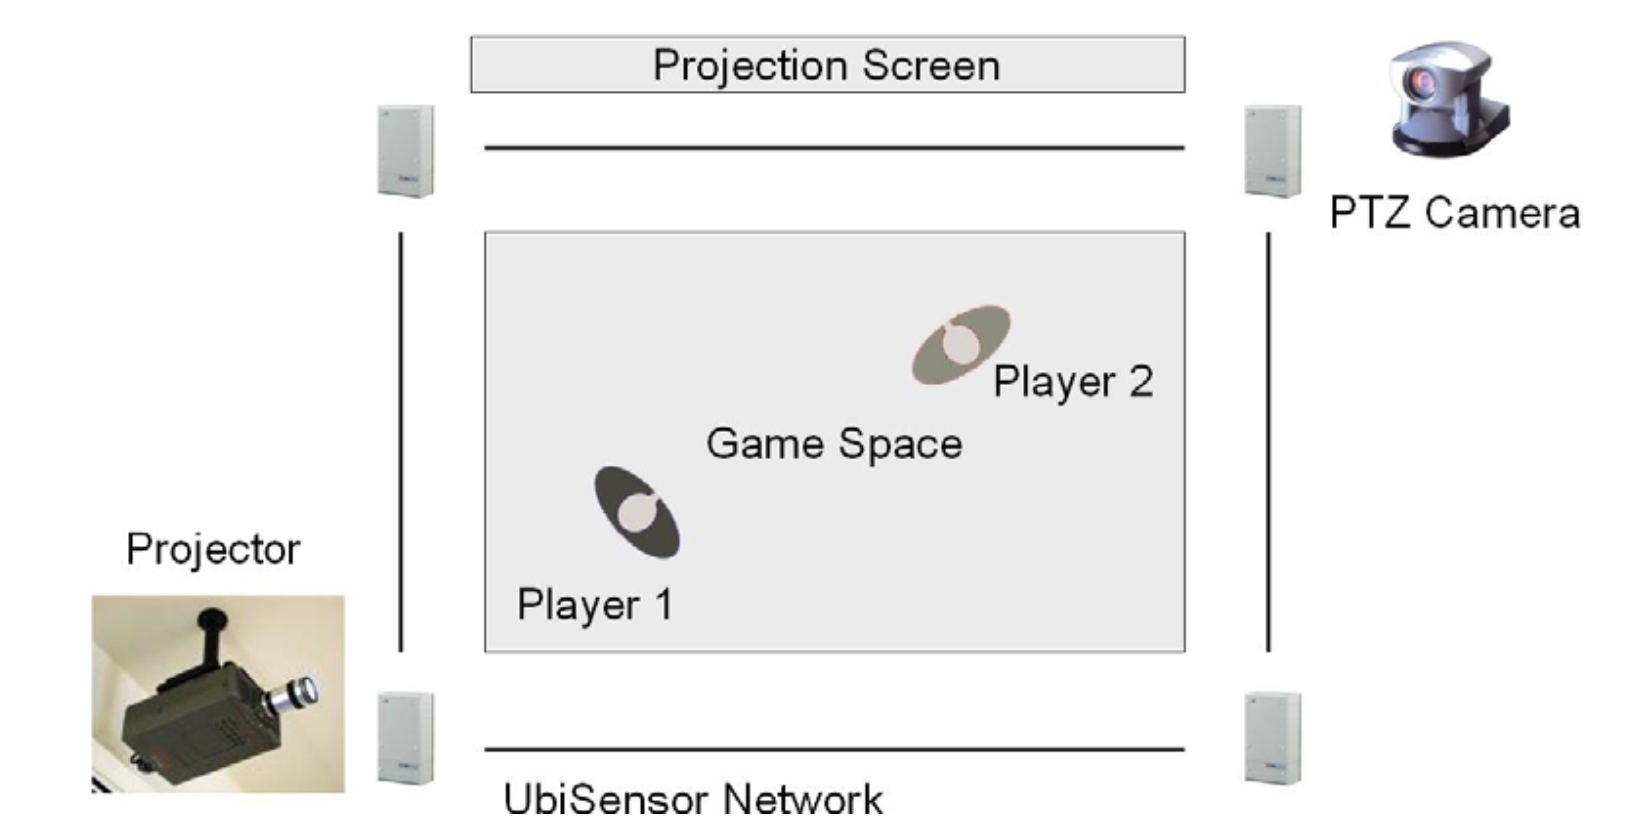
\includegraphics[width=0.5\linewidth]{2.Chapter/ubisense.png}
	\caption[Uisense's system setup (Ref \cite{ubisense}) ]{Uisense's system setup (Ref \cite{ubisense})}
	\label{fig:ubisense}
\end{figure}


\subsection{Other systems}
\label{subsec:others}

\begin{itemize}

\item [] Optical indoor positioning systems are systems that use a camera as their only or main input for position estimation. In recent years these types of systems have found an increase in sucess due to the improvements and size reduction of the sensors, the improvements in computational capacities and the constinuos development of image processing algorithms. Optical systems can be described as a moving sensor, for example a smartphone camera, and oftem times a set of static sensors which detect movement and which utilize \ac{AoA} techniques to estime distances. There are many different types of optical systems, one of them makes use of 3D building models. This approach removes the need for local infrastructure deployment in the building to be monitored since the usualy required refence nodes are replaced by a digital reference point. As such they are highly scalable with small increases in cost.
In general optical systems are capable of achieving high accuracy but they are vulnerable to light conditions, require \ac{LOS} propagations and are more computationally expensive than other types of systems.


\item [] \ac{FM} radio is a broadcasting technology that has been incorporated for a long time on smartphones with the intent of listening to music or to the news. This technology was originaly reserved for frequency modulation to convey information over a carrier wave by varying its frequency but nowadays it just refers to any radio wave in the frquency band 88-108 MHz. This analogue radio signal has amazing advantages for urban/indoor location system such as the ability to be received indoor and outdoor, it has a dense coverage in urban areas, available without installing aditional transmitters, low-cost and low-power hardware with simple technology, high received signal power and there are a large number of transmitters which provides good geometry for locationing. One crucial part when utilizing \ac{FM} is that it doesn't carry any timing information which is critical in range calculation and the fact that as other radio frequency technologies, it suffers from  multipath effects and non-\ac{LOS} signals. An example of FM system was created by  et al. \cite{fm} which implemented an \ac{RSSI} fingerprint-based system using FM radios in an office environment. The system's test bed obtained 17 FM channels at each point of the fingerprint and it was capable of achieving a mean accuracy of 3 meters.


\item [] Zigbee is an emerging wireless technology standard which provides solution for short and medium range communications and its specialy designed for applications which demand low-power consumption and don't require large data throughput. This technology's signal range coverage can go up to 100 meters in open space, while achieving 20 to 30 meters in indoor environments. Most zigbee-based system utilize \ac{RSSI} for distance calculation and one of its most relevant disadvantage is the its vulnerability to interferance from a wide range of signal types using the same frequency which can disrupt radio communication. This is caused by Zigbee operating in the unlicensed ISM (industrial, scientific and medical reserved) bands. An example of a Zigbee-based system is the one created by Larrañaga et al. \cite{zigbee} which attempted to locate a mobile node in an indoor environment. Their system consisted of two phases: The first one, calibration, every existant reference zigbee node transmitted message to each of the remaining. In this ways it was possible to work out the relationship between measured \ac{RSSI} values and geometric distances, allowing to understand the environment moments before attempting a location. The second phase, location, utilizes the data collected and the new data obtained from messages from the mobile user to the refence node to obtain its location. This system was capable of achieved an accuracy with an avarege error of 3 meters.  


\item [] Ultrasonic system are utilized in indoor positioning by making use of \ac{ToA} to locate targets. These kind of system make use of ultrasonic transciever to emit and detect signals while recording times of departure and arrival of the signal. Since the signal medium traveling speed is known, it is possible to use the time difference to compute the distance between emitter and receiver.  One of the most famous projects that makes use of this technology is the cricket system which is described in section \ref{sec:related}.


\item [] Hybrid positioning systems are systems which combine several different positioning technologies to determine the location of a user or object. These types of systems make use of different technologies in an attempt to compensate for one's shortcomings through another's strengths. One example of an hybrid system is the solution presented by versus \cite{versus} which makes use of Wi-Fi, IR and RF to provide a system capable of displaying real-time locations of people or objects inside a building. By combining these three technologies their were capable of providing a system with different level of accuracy depending on the needs, room-level, bed-level (a fragment of a room) or chair-level (precise positioning). 

\end{itemize}
